\documentclass[10pt,a4paper,ngerman]{article}
\usepackage[utf8]{inputenc}
\usepackage{tkz-euclide}
\usepackage[T1]{fontenc}

%\usepackage[]{ntheorem}
%\usepackage[amsthm,thmmarks]{ntheorem}
\usepackage{amsmath}
%\usepackage{amsthm}
\usepackage{hyperref}
\usepackage{cleveref}

\usepackage{amsthm}
\usepackage{thmtools}
\usepackage{amsfonts}
\usepackage{amssymb}
\usepackage{babel}
\usepackage{textcomp}

\usepackage{adjustbox}


\newtheoremstyle{mytheorem}
  {} % Space above (default: 3pt)
  {} % Space below (default: 3pt)
  {\itshape} % Body font: set to italic (standard for plain theorem style)
  {} % Indent amount
  {\bfseries} % Head font: set to bold
  {.} % Punctuation after theorem head (e.g., Theorem 1.1.)
  {.5em} % Space after theorem head (e.g., .5em or " " for normal interword space)
  {\thmname{#1}\thmnumber{ #2}\thmnote{ (\textbf{#3})}}


\theoremstyle{definition}
\newtheorem{defn}{Definition}
\newtheorem*{example}{Beispiel}

\theoremstyle{plain}
\theoremstyle{mytheorem}
\newtheorem{theorem}{Satz}
\newtheorem{lemma}{Lemma}
\newtheorem*{axiom}{Axiom}

\newcommand{\R}{\mathbb{R}}
\newcommand{\N}{\mathbb{N}}
\newcommand{\Q}{\mathbb{Q}}
\newcommand{\Z}{\mathbb{Z}}
\newcommand{\Prim}{\mathbb{P}}
\newcommand{\Nnull}{\mathbb{N}_0}

%*****************************************
\usepackage{adjustbox}
%\usepackage{stackengine}
%\usepackage{paralist}
\usepackage{xfp}
\usepackage{siunitx} % Wichtig für Zahlenformatierung
\usepackage{xparse}
\usepackage{xstring}
\usepackage{enumitem}
\usepackage{environ}
\usepackage{textcmds}
\usepackage[left=25mm,right=25mm,top=25mm,bottom=25mm,paper=a4paper]{geometry}

\usepackage[HTML]{xcolor}


\newcommand{\qref}[1]{\hyperref[#1]{#1}}

\definecolor{c00a0dc}{HTML}{00A0DC}
\definecolor{cbdbdbd}{HTML}{0BBDBD}
\definecolor{ce05022}{HTML}{E05022}
\definecolor{ce5e5e5}{HTML}{E5E5E5}
\definecolor{c7fcfed}{HTML}{C7FCFE}
\usepackage{svg}

\usepackage{siunitx}
\sisetup{locale = DE}
%\usepackage{array}

\theoremstyle{definition}
\newtheorem*{auf}{Aufgabe}

\usepackage{circuitikz}[european]


%\newcommand{\frage}[6]{%
%  \item[#1] #2
%  \begin{enumerate}
%    \item #3
%    \item #4
%    \item #5
%    \item #6
%  \end{enumerate}
%}


%\makeatletter
\NewEnviron{sol}[1]{%
  \edef\macroname{savedata@#1}%
  % Verwende \let anstelle von \edef, um eine Expansion des Inhalts zu verhindern
  \expandafter\global\expandafter\let\csname \macroname\endcsname\BODY
}
%\makeatother

\newcommand{\getsavedata}[1]{%
  \ifcsname savedata@#1\endcsname
    \par\noindent\hrulefill\par
    \textbf{Lösungsansatz:}\par
    \csname savedata@#1\endcsname
    \par\noindent
    \hrulefill%\par
  \else
    % Nichts tun oder eine Warnung ausgeben
  \fi
}

\newcommand{\pic}[2][1]{%
\begin{center}
    \begin{tikzpicture}[scale=#1]
        \input{bilder/#2.tex}        
    \end{tikzpicture}
\end{center}    
}

\newcommand{\qgrafic}[1]{%
\begin{center}
    \begin{tikzpicture}[scale=1.3]
        \input{pic/#1_q.tex}        
    \end{tikzpicture}
\end{center}    
}

% Automatic layout switcher
\newsavebox{\tempbox}
\newlength{\imgwidth}


\newcommand{\agrafic}[2]{%
\resizebox{!}{3cm}{
  \begin{tikzpicture}[scale=1.5]
      \input{pic/#1_#2.tex}        
  \end{tikzpicture}
}
}


\ExplSyntaxOn
\NewDocumentCommand{\frage}{ m m m m m m m m }{
  \item[#1] \label{#1} #2
    \tl_if_eq:nnTF {#7} {true} {
        \qgrafic{#1}
    }{}
\getsavedata{#1}

\tl_if_eq:nnTF {#8} {true} {
\begin{center}

  \sbox{\tempbox}{\adjustbox{valign=c}{\agrafic{#1}{a}}}%
  \settowidth{\imgwidth}{\usebox{\tempbox}}%

  % If two side-by-side images exceed 0.9 of text width, switch to 1x4
  \ifdim 2\imgwidth>0.9\linewidth
    % ---------- Wide layout: 1×4 ----------
    \begin{enumerate}[label=(\Alph*)]
      \item \adjustbox{valign=c}{\agrafic{#1}{a}}
      \item \adjustbox{valign=c}{\agrafic{#1}{b}}
      \item \adjustbox{valign=c}{\agrafic{#1}{c}}
      \item \adjustbox{valign=c}{\agrafic{#1}{d}}
    \end{enumerate}
  \else
    % ---------- Normal layout: 2×2 ----------
    \begin{tabular}{cc}
      (A) \adjustbox{valign=c}{\agrafic{#1}{a}} &
      (B) \adjustbox{valign=c}{\agrafic{#1}{b}} \\
      \multicolumn{2}{c}{\vspace{10pt}} \\
      (C) \adjustbox{valign=c}{\agrafic{#1}{c}} &
      (D) \adjustbox{valign=c}{\agrafic{#1}{d}} \\
    \end{tabular}
  \fi

\end{center}


%\begin{enumerate}[label=(\Alph*)]
%    \item \adjustbox{valign=c}{\agrafic{#1}{a}} 
%    \item \adjustbox{valign=c}{\agrafic{#1}{b}} 
%    \item \adjustbox{valign=c}{\agrafic{#1}{c}} 
%    \item \adjustbox{valign=c}{\agrafic{#1}{d}}   
%  \end{enumerate}        
} {
  \begin{enumerate}[label=(\Alph*)]
    \item #3
    \item #4
    \item #5
    \item #6
  \end{enumerate}      
}

}
\ExplSyntaxOff

\newenvironment{ohmchapter}{}
{
  \subsubsection*{Lösungen}
  \input{tex_sections/\arabic{section}S\arabic{subsection}.tex}
}



\newcommand{\DEnumber}[1]{%
    \num[
        parse-numbers=true,          % Wichtig: Erzwingt die Analyse der Zahl
        output-decimal-marker={,},   % Für das Komma als Dezimaltrennzeichen
        group-separator={\,},        % Optional: Dünner Zwischenraum als Tausender-Trennzeichen
        scientific-notation=false    % Sicherstellen, dass keine wissenschaftliche Notation verwendet wird
    ]{#1}%
}

\newcommand{\calc}[1]{%
  \DEnumber{\fpeval{#1}}
}

\newcommand{\mischer}[2]{%    
    Wir rechnen: 
    \begin{itemize}
      \item \DEnumber{#1} MHz - \DEnumber{#2} MHz = \calc{#1-#2} MHz
      \item \DEnumber{#1} MHz + \DEnumber{#2} MHz = \calc{#1+#2} MHz        
    \end{itemize}  
}

\author{Thomas Fritzsche}
\title{Lernkrücken für den Amateurfunkkurs der Klasse E von A02}
\begin{document}
\maketitle
\tableofcontents

\section*{Einleitung}
In diesem Dokument stellen wir einige Informationen für den Klasse E Aufbaukurs des Ortsverbands A02 zusammen.
Es sei darauf hingewiesen, dass der Author ein Funkamateur im wahrsten Sinne des Wortes ist, und als Amateur keine berufliche Ausbildung im Bereich der hier dargestellten Amateurfunkthemen hat. 

Deshalb kann dieses Dokument inhaltliche Fehler, sachlich falsche Aussagen enthalten. Der Author ist dafür nicht haftbar.
Das Ziel des Dokuments ist auch nicht ein möglichst genaue Fachliche Darstellung der Themen, sondern vielmehr Lernhilfen zu geben, damit die Fragen in der Amateurfunkprüfung der Klasse E richtig beantwortet werden können.

Da sich Funker immer per \qq{Du} ansprechen, will ich in diesem Dokument auch nicht anders machen.

Dieses Dokument verwendet die Kapitalstruktur der DARC Lernplattform \url{http://50ohm.de}. Du kannst also alle Inhalte dort nachlesen. In diesem Dokument fassen wir die Inhalte absichtlich nur sehr knapp zusammen. Wir beschränken uns auf die nach Inhalte die im Fragenkatalog vorkommen. 

Wenn es sich nicht im ein triviale definition handelt wird die Lösung jeder Frage im Detail im Block \qq{Lösungsansatz} erklärt.

\setcounter{section}{7}
\section{Grundlegende Schaltungen}
\setcounter{subsection}{3}
\subsection{Mischer (Klasse E)}

\begin{sol}{EF201}
    \mischer{31.7}{21}  
\end{sol}
\begin{sol}{EF202}
    \mischer{38.7}{28}
\end{sol}
\begin{sol}{EF203}
    \mischer{39}{30} 
\end{sol}
\begin{sol}{EF204}
    \mischer{145}{136} 
\end{sol}
\begin{sol}{EF205}
    \mischer{145}{136} 
\end{sol}
\begin{sol}{EF206}
    In der Frage geht es um \glqq unerwünschte Abstrahlungen\grqq{}, wir müssen also abschirmen.    
\end{sol}


\begin{ohmchapter}
In einem Mischer werden zwei Eingangssignale zu einem Ausgangssignal gemischt. Das Blockschaltdiagramm eines Mischers sieht aus wie eine Waschmaschine. Tatsächlich soll uns das Kreuz in der Mitte des Symbols an ein Multiplikationszeichen erinnern, da es sich um meine multiplikative Mischung von Frequenzen handelt.
Beim Mischen entsteht aus den beiden Eingangsfrequenzen die Summe und Differenz Frequenz:


\begin{center}
\begin{adjustbox}{margin=10pt}
\begin{circuitikz}
\draw (0,0) node[mixer,boxed] (M) {}; 
\draw[->] (-2, 0)node[left] {$f_{\text{in 1}}$} -- (M.w); 
\draw[->] (0, -2)node[below] {$f_{\text{in 2}}$} -- (M.s); 
\draw[->] (M.out) -- (2, 0) node[right,text width=5cm] {
$\begin{aligned}
      &f_{\text{out 1}} = f_{\text{in 1}} + f_{\text{in 2}}\\
      &f_{\text{out 2}} = | f_{\text{in 1}} - f_{\text{in 2}} | 
    \end{aligned}$
    }; 
\end{circuitikz}
\end{adjustbox}
\end{center}



Wie solch ein Mischer funktioniert kannst Du mit dieser \href{https://fritzsche.github.io/klasse-e/mischer.html}{App} interaktiv ausprobieren.


%$$f_{\text{out 1}} = f_{\text{in 1}} + f_{\text{in 2}} \textrm{\ und\ }f_{\text{out 2}} = | f_{\text{in 1}} - f_{\text{in 2}} |$$
%Als Blockschaltdiagramm sieht es folgendermaßen aus:


Hier nur eine kurze Erklärung wie sich dies Mathematisch herleiten lässt. Für die Prüfung brauchst Du diese Details nicht wissen!
In unserem Beispiel haben wir ein empfangenes Signal $S_{\text{empf}}$ 
und das Signal eines lokalen Oszillator  $S_{\text{LO}}$.

% --- Definition der Eingangssignale ---
\begin{align*}
    S_{\text{empf}}(t) &= A_{\text{empf}} \cdot \sin(\omega_{\text{empf}} t) \\
    S_{\text{LO}}(t) &= A_{\text{LO}} \cdot \sin(\omega_{\text{LO}} t)
\end{align*}

Ein Multiplikativer Mixer wird unser Signal zu einem  wie eine einfache Ausgangssignal $S_{\text{out}}$ multiplizieren:

% --- Mischer-Multiplikation ---
\begin{equation*}
    S_{\text{out}}(t) = S_{\text{empf}}(t) \cdot S_{\text{LO}}(t)
\end{equation*}

% --- Produkt-zu-Summe-Formel (Trigonometrie) ---
Wir verwenden die folgende Trigonometrie Formel:
\begin{equation*}
    \label{eq:sin_prod}
    \sin(A) \cdot \sin(B) = \frac{1}{2} \left[ \cos(A-B) - \cos(A+B) \right]
\end{equation*}

% --- Das resultierende Ausgangssignal ---

Also gilt:
\begin{align*}
    S_{\text{out}}(t) &= A_{\text{empf}} A_{\text{LO}} \cdot \sin(\omega_{\text{empf}} t) \cdot \sin(\omega_{\text{LO}} t) \\
    S_{\text{out}}(t) &= \frac{1}{2} A_{\text{empf}} A_{\text{LO}} \left[ \cos((\omega_{\text{empf}} - \omega_{\text{LO}}) t) - \cos((\omega_{\text{empf}} + \omega_{\text{LO}}) t) \right]
\end{align*}

Summe und Differenz entstehen also einfach aus unserer Formel.

% --- Komponenten-Bezeichnung (Optional, als Text) ---
% Die Differenzfrequenz ($\omega_{\text{empf}} - \omega_{\text{LO}}$) ist die Zwischenfrequenz (ZF).


\end{ohmchapter}

\begin{sol}{EF501}
    Der Transverter setzt natürlich vom 70cm Signal ins 10m Band um und umgekehrt.
    Aufpassen bei Antwort (B): Hier wird beim Senden und Empfangen jeweils von 70cm in's 10m Band umgesetzt. Das macht keinen Sinn. 

\end{sol}
\begin{sol}{EF502}
    Im letzten Kapitel haben wir über den Mixer gesprochen. Hier wird Summe und Differenz Frequenz gebildet.
\end{sol}
\begin{sol}{EF503}
    Im Blockschaltbild können wir die Sende-/Empfangsumschaltung erkennen wie zwischen RX und TX umschaltet. Es ist also der \textbf{Transverter}.
\end{sol}

\begin{sol}{EF504}
    Es gibt keine Sende-/Empfangsumschaltung und überhaupt nur den Empfang. Es ist also ein \textbf{Konverter}.
\end{sol}

\begin{sol}{EF505}
    Diese Fragen hat viele ähnlich Antworten. Liess dies alle genau durch!
    Es geht um den Satellitenbetrieb über die hohe Frequenz von 2,4 GHz. Wir müssen also die Sendefrequenz vervielfachen und damit vervielfachen wir auch Frequenzabweichungen.
\end{sol}

\begin{sol}{ED403}
    Die Antwort sollte klar sein, die alternativen Antworten (B),(C),(D) machen überhaupt keinen Sinn.
\end{sol}

\begin{sol}{EF307}
    Hier geht es um Audio Signale vom Mikrofon. Das Menschliche Ohr kann bis maximal ca. 20k Hz hören, allerdings verwenden wird im Amateurfunk nur die untersten 2700Hz davon um nicht unnötig Bandbreite zu verschwenden. Die untersten 300Hz können wir nicht hören, deshalb kann ein Mikrofonverstärker mit der Kennlinie (A) auch als extra Filter dienen. 
\end{sol}

\subsection{Konverter und Transverter}
\begin{ohmchapter}
  Wir müssen Konverter und Transverter unterscheiden können.
  \begin{description}
  \item[Konverter] setzen das Signal nur in eine Richtung um (entweder im Sendepfad oder im Empfangspfad).
  \item[Transverter] verfügen über eine interne Sende-/Empfangsumschaltung und setzen das Signal in Sende- und Empfangsrichtung um (ähnlich wie ein Transceiver).
  \end{description} 
  Wenn also eine \qq{Sende-/Empfangsumschaltung} vorhanden ist, dann ist es ein Transverter.
\end{ohmchapter}

\begin{sol}{ED401}
 Die Frage ist einfach zu beantworten, hat aber mal wider viele ähnlich Antworten.
 Zunächst schließen wir Antwort (C) und (D) aus, da wir ja mit dem Verstärker die Ausgangsleistung erhöhen wollen. Der unterschied von (A) und (B) ist nur ab eine Spannungsquelle notwendig ist und auch dies ist einleuchtend, dass für ein Verstärkung Energie zugeführt werden muss. Deshalb brauchen wir ein Spannungsquelle.  
\end{sol}

\begin{sol}{ED401}
 Die Frage ist einfach zu beantworten, hat aber mal wider viele ähnlich Antworten.
 Zunächst schließen wir Antwort (C) und (D) aus, da wir ja mit dem Verstärker die Ausgangsleistung erhöhen wollen. Der unterschied von (A) und (B) ist nur ab eine Spannungsquelle notwendig ist und auch dies ist einleuchtend, dass für ein Verstärkung Energie zugeführt werden muss. Deshalb brauchen wir ein Spannungsquelle.  
\end{sol}

\begin{sol}{ED402}
 In der Schaltung finden wir ganz Zentral den Transistor, der ja typisch ist für den Verstärker, also schließen wir schon mal (D) aus. Weiterhin finden wir das Schaltzeichen eines Lautsprechers im Schema, es geht also um Audio (NF).   
\end{sol}

\begin{sol}{EF308}
  Bereits aus der Frage erfahren wir, dass es um einen NF-Verstärker geht, auch wenn zur Verwirrung noch Mixer und Bandpass eingezeichnet sind. Die Bezeichnungen SSB und LSB/USB lässt uns erkennen, dass es um das gewünschte Audiospektrum von ca. 2,5 kHz geht.
\end{sol}

\begin{sol}{EF403}
 Wichtig ist, dass wir uns merken, dass ein SSB Verstärker die Signale \textbf{linear} verstärken soll. Er muss dabei z.B. die gesamte Bandbreite des Signals gleichmäßig abdecken und sollte nicht bei gewünschten Frequenzen (SSB) oder Amplituden einbrechen (die Amplitude eines SSB Signals hängt von der Lautstärke des NF Signals ab).
\end{sol}

\begin{sol}{EF405}
  Die Stromversorgung in einem Sender, sollte niederohmig sein, um eine stabile und effiziente Energieversorgung der Senderendstufe zu gewährleisten. Die Antwort (C) und (D) macht ebenso keinen Sinn. Also merken wir uns, dass wir keine HF in der Stromzufuhr haben wollen. Bei Netzversorgung würden wir ja sonst auch die HF über das Stromnetz in der ganzen Nachbarschaft verteilen.
\end{sol}

\subsection{Verstärker}
\begin{ohmchapter}
Der Transistor ist für moderne Verstärker das Entscheidende Bauelement, dass uns hilft die Schaltungen aufeinander halten zu können. Für viele Jahre wurden auch Röhren verwendet, die auch heute noch viele Amateurfunker verwenden. Allerdings kommen sie nicht mehr im Fragenkatalog vor.
\end{ohmchapter}  


\section{Modulation} \label{sec:modulation}
\subsection{Unmodulierter Träger}


\begin{sol}{EE101}
  In (A) haben wir einen unmodulierten Sinus. (B) ist Frequenzmoduliert (C) ist Phasenmoduliert und (D) ist Amplitudenmoduliert. Schau Dir einfach an was sich abweichend von einem Sinus Signal in den Diagrammen ändert.
\end{sol}

\begin{ohmchapter}
  Der unmodulierter Träger entspricht im zeitlichen Verlauf eine Sinus Funktion.

\end{ohmchapter}  

\subsection{Einseitenbandmodulation (SSB)}

\begin{sol}{EE201}
  SSB unterscheidet sich von AM dadurch, dass nur eins von den beiden Seitenbändern hat und keinen Träger. In Bezug auf die Bandbreite ist es deshalb nur etwa halb so breit. Ansonsten unterscheidet sich SSB von AM nicht, Du kannst mit einem SSB Empfänger AM Empfangen, in dem Du deinen Empfänger auf jeweils eines der Seitenbänder einstellst.
\end{sol}

\begin{sol}{EE202}
  Die Bandbreite des NF Signals überträgt sich auf das HF Signal. Praktisch für Dich in der Prüfung, es gibt einige Fragen zur Bandbreite von NF und/oder SSB die nur minimal abweichen. Bei 2,4 kHz - 2,7 kHz liegst Du also fast immer richtig.

\end{sol}

\begin{sol}{EE203}
  Wir addieren, da das Signal im oberen Seitenband liegt (USB). Pass mit MHz bzw. KHz auf!
  
  Rechnung: 21,250Mhz + 1 kHz = 21,251 MHz 
\end{sol}

\begin{sol}{EE204}
  Wir subtrahieren, da das Signal im unteren Seitenband liegt (LSB). Pass mit MHz bzw. kHz auf!
  
  Rechnung: 3,65 Mhz + 2 kHz = 3,648 MHz 
\end{sol}


\begin{sol}{EE205}
  Die Amplitude des NF Signal regelt bei SSB die Ausgangsleistung. Wenn wir die Ausgangsleistung reduzieren wollen sollten wir die Amplitude des NF Signals reduzieren.
\end{sol}
\begin{sol}{EE206}
  Die Amplitude des NF Signal regelt bei SSB die Ausgangsleistung. Wenn unsere Mikrofonverstärkung nicht ausreicht haben wir auch nur eine geringe Ausgangsleistung.
\end{sol}
\begin{sol}{EE207}
  CW hat eine deutliche geringere Bandbreite als Sprachsignale via SSB oder AM. Deshalb ist es deutlich effektiver und erfreut sich großer Beliebtheit der der Welt des Amateurfunk.
\end{sol}

\begin{sol}{EF310}
Wie bei vielen anderen SSB Fragen ist die Antwort um 2,5 kHz richtig, also (A)!
\end{sol}


\begin{sol}{EJ210}
Wie bei vielen anderen SSB Fragen ist die Antwort um 2,5 kHz richtig, also (A). In dieser Frage liegt der Wert bei 2,7 kHz noch ca. 300 Hz zum (gefilterten) Träger Abstand sind. Dies entspricht den tiefen NF Frequenzen die wir Menschen nicht hören können.
\end{sol}

\begin{sol}{EJ215}
 Eine zu hohe Mikrofonverstärkung führt zu einer Übersteuerung der Verstärkerendstufe und zu Splatter auf die Nachbarfrequenzen.  Zudem machen wir es unserem Filter schwerer die Frequenzen außerhalb des Bandpass-Filter zu unterdrücken.
\end{sol}

\begin{ohmchapter}
  Wir haben die SSB Modulation bereits im Klasse N Kurs kennengelernt. Ein SSB Signal entspricht im Grunde der Amplitudenmodulation AM, bei der der Träger und ein Seitenband unterdrückt werden.
  
  Im Amateurfunk verwenden wir in der Regel die Audio Frequenzen von 300 Hz bis 3000 Hz, dies entspricht also in etwa 2.7 kHz. Auch die Bandbreite des ausgesendeten HF Seitenbandes ist in etwas so groß. Es gibt im Katalog viele Fragen zur Bandbreite von SSB oder des NF Signals die Du alle mit der Antwort um die 2.5-3 kHz richtig beantwortest.
  \pic[1.3]{ssb}
\end{ohmchapter}  

\subsection{Frequenzmodulation (FM)}
\begin{sol}{EE301}
  In diesem Bild ändert sich die Frequenz des Signals, wie sehen also FM.
\end{sol}

\begin{sol}{EE302}
  Schon beim Empfang von FM Rundfunk hast Du bestimmt bemerkt, dass FM klarer klingt. Das liegt u.A. daran dass FM nicht von der Amplitude abhängt, die von vielen Einflüssen z.B. in der Atmosphäre (QRN / QRM) beeinflusst wird.
  Früher haben auch die Zündung in Automotoren für Störungen in AM gesorgt, die mit FM nicht auftreten.
\end{sol}

\begin{sol}{EE303}
  FM wie in Frage EE302.
\end{sol}

\begin{sol}{EE304}
  Der Frequenzhub gibt an wie weit (Frequenz) der der Träger moduliert wird. Deshalb führt ein großer Frequenzhub zu einer großen HF Bandbreite.
\end{sol}

\begin{sol}{EE305}
 Wir müssen den Frequenzhub reduzieren.
\end{sol}

\begin{sol}{EE306}
  Wie der Name Frequenzmodulation (FM) bereits impliziert wird die Lautstärke (NF Amplitude) über die Trägerfrequenzauslenkung moduliert.  
\end{sol}

\begin{ohmchapter}
  Wie der Name Frequenzmodulation (FM) bereits verrät wird beim FM die Frequenz des HF Trägers moduliert (verändert). Der Hub gibt an wie weit die Frequenz von der Grundfrequenz abgelenkt wird. Hier wird das NF Signal und die entsprechende Auslenkung des HF Trägers gezeigt:
  \pic[0.8]{fm}
  Da FM über die Frequenz moduliert wird ist FM \textbf{unempfindlicher gegenüber Amplitudenstörungen}. 
\end{ohmchapter}  

\subsection{Bandbreite}
\begin{sol}{EA105}
  In Hertz (Hz).
\end{sol}

\begin{ohmchapter}
\end{ohmchapter}  

\subsection{Dynamikkompressor}

\begin{sol}{EF306}
  Da SSB von der Amplitude des NF (Audio) Signals abhängt, gebt der Dynamikkompressor schwache Audio Anteile an um ein stärkeres und klarer verständlicheres Signal zu erzeugen. Ist der Dynamikkompressor zu hoch eingestellt klingt das Signal aber unnatürlich und übermoduliert.
\end{sol} 
\begin{ohmchapter}
\end{ohmchapter}  
\section{Empfänger}
\subsection{Detektorempfänger}
\begin{ohmchapter}
  Das in Frage EF101 gezeigte Schaltbild zeigt bereits alles was einen Detektorempfänger ausmacht. Wir haben keine externe Spannungsversorgung. Die Antenne fängt das HF Signal ein. Variabler Kondensator und eine Induktivität (Spule) bilden ein \textbf{Parallelschwingkreis} und selektieren die gewünschte Frequenz.
  Das Signal wird über eine Diode \textbf{gleichgerichtet}. Durch die Trägheit eines (hochohmigen) Kopfhörers wird ein hörbares NF Signal erzeugt.
  Die Nachteile sind klar: ohne Verstärker können nur sehr starke (AM) Stationen empfangen werden. Der Parallelschwingkreis ist sehr ungenau es wird ein großer Teil des Frequenzspektrums empfangen.
   Dennoch auch heute noch ein faszinierendes Bastelprojekt.
  
\end{ohmchapter}  


\begin{sol}{EF102}
  Die Zwischenfrequenz eines Überlagerungsempfänger hat hat den Vorzeit, dass mit speziellen Filtern eine höhere \textbf{Trennschärfe} erreicht werden kann.s
\end{sol} 

\begin{sol}{EF208}
 Der Direktempfänger mischt das HF Signal direkt auf Audiofrequenz NF. Im Mischer wird die Tatsache ausgenutzt, dass die Differenz der Frequenzen im gemischten Ausgang erzeugt wird. 
 Wenn jetzt Empfangsfrequenz und HF annähernd die selbe Frequenz haben kommt man also in der Differenz in den NF Bereich.
\end{sol} 


\subsection{Überlagerungsempfänger (Einfachsuper)}
\begin{ohmchapter}
  Wir haben im letzten Kapitel mit dem Detektorempfänger ein Beispieleines sogenannten \textbf{Geradeausempfänger} kennengelernt.
  Hier entsteht die Audio Frequenz direkt aus der HF. 
  Üblicher weise wird die HF direkt auf Audio Frequenz gemischt. Deshalb spricht man auch von einem \textbf{Direktüberlagerungsempfänger}.
  Es ist jedoch üblich zunächst auf eine feste \textbf{Zwischenfrequenz} zu mischen. Diese Art von Empfänger nennt man Überlagerungsempfänger.
  Der Vorteil besteht einer festen Zwischenfrequenz besteht darin, dass speziell für diese Zwischenfrequenz optimierte Filter verwendet werden können, z.B. für CW mit nur 300 Hz oder SSB mit 2400 Hz. Dadurch ergibt sich eine bessere \textbf{Trennschärfe}.
  \par
  \pic[0.8]{receiver} 
\end{ohmchapter}  
\subsection{Trennschärfe I }
\begin{ohmchapter}
Je kleiner die Empfangsbandbreite ist, desto enger ist auch mein Filter und das Signal wird deutlich besser. D.h. eine schmale Empfängerbandbreite führt zu einer hohen \textbf{Trennschärfe}. Für guten Empfang ist also eine schmale Bandbreite von Vorteil. Deshalb sind schmalbandige Übertragungsverfahren effektiver. Vergleiche z.B. CW mit SSB. 
\end{ohmchapter}  

\subsection{BFO I}

\begin{sol}{EF217}
  Seht starke Signale können einen Empfänger überlasten und müssen gedämpft werden. Dazu verwenden wir ein \textbf{Dämpfungsglied}.
\end{sol} 

\begin{ohmchapter}
Mit dem \qq{Beat Frequenz Oscillator} (BFO) wird in Überlagerungsempfänger die ZF auf Audio gemischt und damit hörbar gemacht.
\end{ohmchapter}  
\subsection{Vorverstärker und Dämpfungsglied}



\begin{sol}{EF218}
Im UHF (Ultra Hoch Frequenz) sind die Verluste auf den Zuleitungen besonders hoch. Im schlimmsten Fall ist das Nutzsignal durch diese Dämpfung bereits komplett im Rauschen verschwunden. Deshalb werden HF (Vor-)Verstärker im UHF Bereit möglichst direkt an der Antenne montiert.
\end{sol} 

\begin{ohmchapter}
\end{ohmchapter}  

\subsection{Automatische Verstärkungsregelung (AGC) I} \label{agc}
\begin{ohmchapter}
  \textbf{AGC} steht für Automatic Gain Control oder auf Deutsch auch Automatische Verstärkerregelung. 

  Sie steuert der HF Verstärker automatisch nach. Wenn sehr starte Signale empfangen werden reduziert die AGC die Verstärker Leistung, wenn die Signale schwach sind regelt die AGC die Verstärkung nach oben.
  Dadurch wird das NF signal stabiler.

  Achtung: Die AGC regelt den Empfänger. Es gibt eine Verstärkerregelung für den Sender (ALC), diese solltest Du in der Prüfung nicht verwechseln.
\end{ohmchapter}  

\subsection{Notch-Filter}
\begin{sol}{EF216}
Der Notchfilter ist ein Kerb-filter, d.h. er filtert nur einen kleinen Teil des Frequenzspektrums heraus, lässt den übrigen Teil des NF Spektrums durch. Es ist also die Kerbenform von (A).
\end{sol} 
\begin{ohmchapter}
Sehr \textbf{schmalbandige Störungen} (QRM) können mit einem Kerbfilter auch \textbf{Notch-filter} eliminiert werden.
\end{ohmchapter}



\subsection{Rauschunterdrückung}
\begin{ohmchapter}
  Die \textbf{Rauschunterdrückung}, auch auf Englisch als Noise Reduction(NR) benannt dient der Unterdrückung von Rauschen.
  Der \textbf{Noise Blanker} hingegen eliminiert impulsartige Störungen, wie sie z.B. früher von Motor Zündungen erzeugt wurden.
\end{ohmchapter}  


\subsection{Frequenzmessung I}


\begin{sol}{EI502}
Der Zähler zeigt MHz an. Dies bezieht sich auf den Punkt hinter der Ziffer 5.
Wir Zählen die Stellen durch:
\begin{itemize}
  \item $5 \cdot \SI{1} {\mega\hertz}$
  \item $0 \cdot \SI{100} {\kilo\hertz}$
  \item $0 \cdot \SI{10} {\kilo\hertz}$  
  \item  $\underbrace{1 \cdot \SI{1} {\kilo\hertz}}_{\text{Stelle mit X}}$
\end{itemize}
\end{sol} 

\begin{sol}{EI503}
Der Zähler zeigt MHz an. Dies bezieht sich auf den Punkt hinter der Ziffer 5.
Wir Zählen die Stellen durch:
\begin{itemize}
  \item $5 \cdot \SI{1} {\mega\hertz}$
  \item $0 \cdot \SI{100} {\kilo\hertz}$
  \item $0 \cdot \SI{10} {\kilo\hertz}$
  \item $1 \cdot \SI{10} {\kilo\hertz}$
  \item $3 \cdot \SI{100} {\hertz}$
  \item $\underbrace{7 \cdot \SI{10} {\hertz}}_{\text{Stelle mit X}}$
\end{itemize}
\end{sol} 

\begin{sol}{EI504}
 Ein 10:1 Frequenzteiler hat die Frequenz um einen einen Faktor 10 reduziert, aus \SI{10}{\mega\hertz} wurde \SI{1}{\mega\hertz} in der Anzeige.
 Für die Aufgabe müssen wir den angezeigten Wert mit 10 multiplizieren.
 $$ \SI{14,5625}{\mega\hertz} \cdot 10 = \SI{145,625}{\mega\hertz}$$
 Check: die Frequent liegt im 2-Meter Amateurfunkband.
\end{sol}  


\begin{ohmchapter}
Frequenzzähler sind nützliche Messgeräte die, wie der Name bereits andeutet, um die Frequent eines Signals zu messen. Genauer gesagt: die Frequenz eines unmodulierten Hochfrequenzsignals.  Dies kann z.B. genutzt werden um die Frequenz z.B. eines lokalen Oszillator (LO) zu bestimmen.  
\end{ohmchapter}  


\section{Sender}
\subsection{ALC}
\begin{ohmchapter}
Wir haben bereits im Kapitel \ref{agc} über die AGC gesprochen. Dies ist eine automatische Verstärker Steuerung für den Empfänger.
Aber auch der Sender hat hat solch eine Steuerung: Automatic Level Control (ALC). Wie Du im Kapitel über SSB gelernt hast hängt hier die Signalstärke von der Amplitude des NF Signals ab, welches ganz natürlich schwankt wenn wir in das Mikrofon sprechen. 
Um diese Schwankungen entgegenzuwirken und damit die Endstufe zu schützen, reduziert die ALC Signalstärke (Amplitude) wenn sie über ein definiertes Limit geht.
\end{ohmchapter}  
\subsection{Senderausgangsleistung}

\begin{sol}{EF401}
Die \qq{Ausgangsleistung} ist natürlich die Leistung direkt am Senderausgang (vor Zusatzgeräten). Vor- bzw. rücklaufende Leistung spielen keine Rolle.
\end{sol}  
\begin{sol}{EF402}
Die Peak Envelop Power (PEP) oder auf Deutsch maximale Hüllkurvenleistung wird direkt am Senderausgang gemessen.
Mit der Klasse E sind oft 100 W zulässig. Eine Antenne mit Gewinn kann die Abstrahlung noch verstärken.
\end{sol}  

\begin{sol}{EJ209}
Hier geht es mit die Leistung die zu unerwünschten Aussendungen führt. Deshalb wird hier auch Stehwellenmessgerät und ggf. ein verwendeter Tiefpassfilter berücksichtigt werden.
\end{sol}  


\begin{ohmchapter}
  Die Definitionen der Senderausgangsleistung musst Du Dir einfach merken. Wie Du bereits bei der Klasse N gelernt hast, bist Du als  Funkamateur verpflichtet dich an entsprechende Grenzwerte zu halten.
\end{ohmchapter}

\subsection{Unerwünschte Aussendungen II}

\begin{sol}{EJ201}
Nur sinusförmige Schwingungen haben keine Oberwellen. In dieser 
\href{https://fritzsche.github.io/klasse-e/oberwelle.html}{App} kannst Du ausprobieren welche Oberwellen unterschiedliche Signale haben.

\end{sol}  

\begin{sol}{EF404}
Wenn die Senderendstufe neu eingestellt wurde wollte zur Sicherheit überprüft werden, dass keine Oberwellen entstehen.
Wenn nach der Einstellung z.B. kein reiner Sinus mehr erzeugt wird sind Oberwellen dabei.
\end{sol}  


\begin{sol}{EJ202}
Hochfrequente Störungen durch Harmonische werden durch Tiefpassfilter gefiltert. Hier wird explizit nach einen Oberwellenfilter gefragt. Nicht irritieren lassen!
Die Frage EJ203 wird der Begriff Tiefpassfilter verwendet.
\end{sol} 

\begin{sol}{EJ203}
In dieser Fragen finden wir schnell, dass uns ein Tiefpassfilter hilft.
Du kannst einen Tiefpassfilter in dieser \href{https://fritzsche.github.io/klasse-e/lpf.html}{App}
praktisch ausprobieren, in dem ein Rechtecksignal durch bei geeigneten Parametern durch einen Tiefpassfilter zu einem Sinus Signal wird.
\end{sol}  

\begin{sol}{EJ204}
Der Tiefpassfilter ist mal wieder die richtige Antwort.
\end{sol}  


\begin{sol}{EJ205}
Auch für UHF Sender wird man einen Tiefpassfilter verwenden, wenn man Oberwellen unterdrücken will.
\end{sol}  


\begin{sol}{EJ206}
Es gibt mehrere Fragen nach denen dem Schaltbild eines Filters gefragt wird. Bei all Fragen kann man sich die Position des Kondensators im Vergleich zur Spule ansehen. Ist der Kondensator \qq{unten} so handelt es sich um einen Tiefpass, sonst om einen Hochpass.
Da Oberwellen mit einem Tiefpassfilter gedämpft werden bleibt nur diese Antwort.
\end{sol}  

\begin{sol}{EJ206}
Es gibt mehrere Fragen nach denen dem Schaltbild eines Filters gefragt wird. Bei all Fragen kann man sich die Position des Kondensators im Vergleich zur Spule ansehen. Ist der Kondensator \qq{unten} so handelt es sich um einen Tiefpass, sonst om einen Hochpass.
Da Oberwellen mit einem Tiefpassfilter gedämpft werden bleibt nur diese Antwort. Beachte bitte, dass dies natürlich im allgemeinen nicht gild, da es davon abhängt wie der Schaltplan gezeichnet wurde, aber die Schaltpläne des aktuelle Fragekatalogs wurden alle so gezeichnet, dass die Regel gilt. 
\end{sol}  


\begin{sol}{EJ207}
Ein Filter zur Verringerung von Oberwellen ist ein Tiefpassfilter. D.h. die Tiefen Frequenzen werden ungehindert durchgelassen, die hohen Frequenzen werden abgeschwächt.
In der Frage geht es um einen Kurzwellen-Sender, d.h. wir wollen alle Frequenzen unterhalb von \SI{30}{\mega\hertz} durchlassen und nur oberhalb filtern. Dies finden wird in Bild A.
\end{sol}  


\begin{sol}{EJ208}
Wie bei Frage EJ207: Ein Filter zur Verringerung von Oberwellen ist ein Tiefpassfilter. D.h. die Tiefen Frequenzen werden ungehindert durchgelassen, die hohen Frequenzen werden abgeschwächt.
In der Frage geht es um einen Kurzwellen-Sender, d.h. wir wollen alle Frequenzen unterhalb von \SI{30}{\mega\hertz} durchlassen und nur oberhalb filtern. Dies finden wird in Bild A.
\end{sol}  

\begin{ohmchapter}
  Unerwünscht Aussendungen entstehen oft durch \textbf{Oberwellen}. Diese können in der Regel durch einen \textbf{Tiefpassfilter} vermieden werden.
\end{ohmchapter}


\subsection{Störende Beeinflussung elektronischer Geräte I}


\begin{sol}{EJ101}
Siehe Definition am Anfang des Kapitel.
\end{sol}  

\begin{sol}{EJ102}
Siehe Definition am Anfang des Kapitel.
\end{sol}  


\begin{sol}{EJ103}
Das Schlüsselwort ist \textbf{Übersteuerung}. D.h. das Signal ist einfach zu stark und überlasten den Empfänger in der Nähe.
\end{sol}


\begin{sol}{EJ104}
Dies ist leider ein Grundsatz der oft zu wenig berücksichtigt wird. 
\end{sol}

\begin{sol}{EJ105}
Nicht mit unnötig hoher Sendeleistung zu senden lohnt sich immer.
\end{sol}

\begin{sol}{EJ106}
Mit hohem Gewinn senden wir ein Signal in der Nachbarschaft von TV Kanälen aus. Dies kann den Empfänger im TV Gerät übersteuern.
\end{sol}

\begin{sol}{EJ107}
Bei sehr starken Signalen wird ein Empfänger (z.B. AGC) die Verstärker zurückfahren um eine Übersteuerung zu vermeiden.
Deshalb geht die Empfindlichkeit zurück.
\end{sol}

\begin{sol}{EJ108}
Das Abschirmgehäuse ist in der Regel aus Metall um unerwünschte Aussendungen abzufangen.
\end{sol}

\begin{sol}{EJ109}
Ohne Abschirmung können HF Signale in die 230 V Wechselstromleitung gelangen und dann über die Leitung in andere Geräte einströmen.
\end{sol}


\begin{sol}{EJ111}
Diese Frage lässt sich gut durch das Ausschlussprinzip beantworten. Aber auch direkt mach es Sinn eine getrennte HF Erdung zu verwenden.
\end{sol}

\begin{sol}{EJ112}
Einströmung via Netzanschluss.
\end{sol}

\begin{sol}{EJ113}
Die abgeschaltete Stereoanlage verhält sich hier wir ein Detektorenempfänger. 
\end{sol}

\begin{sol}{EJ114}
Geschirmte Laubsprecherbkabel können Einstrahlungen reduzieren.
\end{sol}

\begin{sol}{EJ115}
Abschirmen.
\end{sol}


\begin{sol}{EJ116}
Die Frequenz von \SI{28} {\mega\hertz } liegt im 10 m Band am oberen Ende der Kurzwelle. Dies sollte aus der Klasse N noch bekannt sein. Die TV Signale liegen vie höher. Wir wollen also hohe Frequenzen durchlassen (TV) aber die niedrigen HF Signale unterdrücken. Wir brauchen also einen Hochpassfilter.
\end{sol}


\begin{sol}{EJ117}
Wie in Frage EJ116 brauchen wir einen Hochpassfilter. Nach der Merkregel sind bei einem Hochpass Filter die Kondensatoren auch oben. Also Schaltbild A.
\end{sol}

\begin{sol}{EJ118}
Eine so genannte Mantelwellensperre oder auch Mantelwellendrossel reduziert Gleichtaktströme. Dies ist HF die sich z.B. auf dem Außenmantel von Koaxialleitungen bilden könnte.
\end{sol}

\begin{sol}{EJ119}
Wie in EJ118 kann eine Mantelwellendrossel diese unerwünschten Gleichtaktströme verringern und muss in das Koax vor dem Empfänger eingebaut werden.
\end{sol}


\begin{sol}{EJ120}
Es werden Mischfrequenzen erzeugt, Phantomsignale. Wir haben bereits über den Mischer gesprochen und eine der Frequenzen abgeschaltet wird verschwindet natürlich auch das Signal.
\end{sol}

\begin{sol}{EJ121}
Wir merken uns die Antwort.
\end{sol}

\begin{sol}{EJ122}
Das einfachste zuerst! Passen die Störungen überhaupt zeitlich zum Funkbetrieb?
Es ist bereits oft vorgekommen, dass die Störungen auftreten obwohl wohl die Amateurfunkanlage nicht in Betrieb war.
\end{sol}

\begin{sol}{EJ124}
Eine Zimmerantenne ist für den Empfang nicht optimal und führen zu einem schlechten Signal Rauschabstand. Durch sind im Verhältnis auch die Störungen viel Stärker (siehe auch AGC). Eine AUßenantenne kann die Situation verbessern.
\end{sol}

\begin{sol}{EJ212}
AFSK (Audio Frequency Shift Keying) wirkt hier wie FM. Durch absenken des audio Pegel reduzieren wir also die Bandbreite.
\end{sol}

\begin{sol}{EJ213}
Ist der Leistungsverstärker übersteuert, so sieht das Signal nicht mehr wie ein Sinus sondern eher wie ein Rechtecksignal. Dies führt zu viel Oberwellen. Aber auch Benachbarte Frequenzen werden durch sogenannte Splatter beeinflusst.
\end{sol}

\begin{sol}{EJ214}
Insbesondere im SSB Bereich sind Splatter (Störungen auf Nachbarfrequenzen) zu beobachten, wenn die Leistungsendstufe übersteuert wird. In einem modernen SDR Transceiver kann man sofort erkennen, dass dabei die 
übliche Bandbreite von ca. \SI{2.4} {\kilo\hertz }  deutlich überschritten wird.
\end{sol}

\begin{sol}{EJ216}
  Die Antwort sollte unmittelbar klar sein.
\end{sol}


\begin{ohmchapter}
Auch in diesem Kapitel geht es um unterschiedliche Störungen die mir einem Sender verursacht werden können.
Wir unterscheiden zwei unterschiedliche Arten von Störungen.

\begin{description}
  \item[Einströhmungen] Die Störung, bzw. die HF wird durch eine Zuleitung, z.B. Netzzuleitung, Antennenzuleitung, Lautsprecherkabel etc. verursacht. 
  \item[Einstrahlung] Die HF gelangt direkt in der gestörte Gerät, z.B. da die Abschirmung nicht ausreicht.
\end{description}

\end{ohmchapter}

\section{Digitale Übertragungsverfahren}
\subsection{Binäres Zahlensystem} \label{sec:binär}



\begin{sol}{EA202}
  Wir haben also 3 Bits. Wir können die Zahl $111_2$ berechnen:
    \begin{center}
  \begin{tabular}{|c|c|c|c|c|c|c|c|} 
    128& 64&32&16 &8 & 4 & 2 & 1 \\ \hline
    0&0&0&0&0&1&1&1
  \end{tabular} 
  \end{center}
Also $111_2 = 4+2+1 = 7$. Dies ist aber keine der möglichen Antworten! Wir haben die 0 vergessen, es wurde ja nach \qq{unterschiedliche(n) Zuständen} gefragt! Also ist 8 die richtige Antwort.

Es geht auch einfacher $1000_2$ die nächst höhere Zahl ist können wird direkt mit $8 = 2^3$ antworten.
\end{sol}


\begin{sol}{EA203}
Analog zu Frage \qref{EA202} rechnen wir $2^4 = 16$.
\end{sol}

\begin{sol}{EA204}
Analog zu Frage \qref{EA202} rechnen wir $2^5 = 32$.
\end{sol}


\begin{sol}{EA205}
  Wir rechnen:
  \begin{center}
\begin{tabular}{|c|c|c|c|c|c|c|c|} 
128& 64&32&16 &8 & 4 & 2 & 1 \\ \hline
0&1&0&0&1&1&1&0
\end{tabular}

\end{center}
Also: $64+8+4+2 = 78$ 
\end{sol} 

\begin{sol}{EA206}
  Wir rechnen:
  \begin{center}
\begin{tabular}{|c|c|c|c|c|c|c|c|} 
128& 64&32&16 &8 & 4 & 2 & 1 \\ \hline
1&0&0&0&1&1&1&0
\end{tabular}

\end{center}
Also: $128+8+4+2 = 142$ 
\end{sol}  


\begin{sol}{EA207}
  Wir rechnen:
  \begin{center}
\begin{tabular}{|c|c|c|c|c|c|c|c|} 
128& 64&32&16 &8 & 4 & 2 & 1 \\ \hline
1&0&0&1&1&1&0&0
\end{tabular}
\end{center}
Also: $128+16+8+4 = 156$ 
\end{sol}  


\begin{sol}{EA208}
  Wir rechnen:
  \begin{center}
\begin{tabular}{|c|c|c|c|c|c|c|c|} 
128& 64&32&16 &8 & 4 & 2 & 1 \\ \hline
1&1&1&1&1&0&0&0
\end{tabular}
\end{center}
Also: $128+64+32+16 = 248$ 
\end{sol}  

\begin{ohmchapter}
  Wir verwenden im Alltag üblicherweise Zahlen im Dezimalsystem. D.h wir verwenden die Ziffern 0 bis 9 alle Zahlen darzustellen. 
  In der Digitaltechnik hat sich allerdings hauptsächlich das Binärsystem durchgesetzt in dem nur die Ziffern 0 und 1 verwendet werden, die durch zwei Zustände (Strom ist ein oder aus) abgebildet werden können.  Das Binärsystem wird manchmal auch Dualsystem genannt.
   Eine Ziffer die im Binärsystem (0 oder 1) wird auch Bit genannt.
  Üblicherweise fassen wir 8 Bit zu einer Zahl zusammen und nennen es Byte.
  Für die Stellen einer 8 Bit Zahl gilt: 
  \begin{align*}
    2^7 &= 128 \\         
    2^6 &= 64 \\
    2^5 &= 32 \\  
    2^4 &= 16 \\         
    2^3 &= 8  \\
    2^2 &= 4 \\         
    2^1 &= 2  \\   
    2^0 &= 1  
  \end{align*}  
Tipp für die Prüfung: viele Schul-Taschenrechner (nicht programmierbar und deshalb vielleicht von der Bundesnetzagentur für die Prüfung akzeptiert) können zwischen Zahlsystemen umrechnen.
\end{ohmchapter}


\subsection{Digimode per SSB}

\begin{sol}{EE402}
  Wie im Eingang zu diesem Kapitel beschrieben wird in der Regel SSB verwendet.
\end{sol}


\begin{sol}{EE403}
Wie bereits im Kapitel zur Modulation erklärt sind bei SSB NF unf HF Bandbreite identisch.
\end{sol}


\begin{sol}{EE404}
Über die Audio Schnittstelle wird am PC die komplette Bandbreite von \SI{2.4}{\kilo\hertz} empfangen. 
Digitale Signale haben oft eine Bandbreite von nur wenigen Hertz und können somit gleichzeitig empfangen werden.
Hier ein Bild eines Wasserfalls mit Spektrum. Im Audio Empfangsbereich liegen viele Signale:
  \begin{center}
    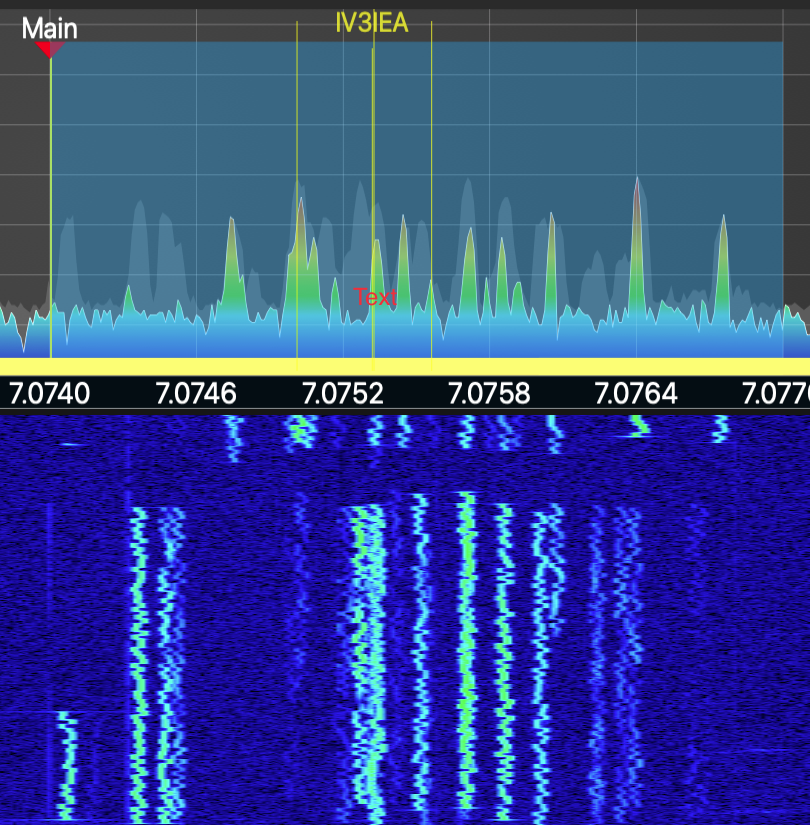
\includegraphics[scale=.5]{bilder/ft8.png}    
  \end{center}
\end{sol}

\begin{sol}{EE415}
  Du musst die einfach merken, dass SSTV (Slow Scan TV) Bilder sind. Diese werden z.B. auch von der ISS im \SI{2}{\meter}  Band gesendet. Hier als Anschauung ein SSTV Bild:
  \begin{center}
    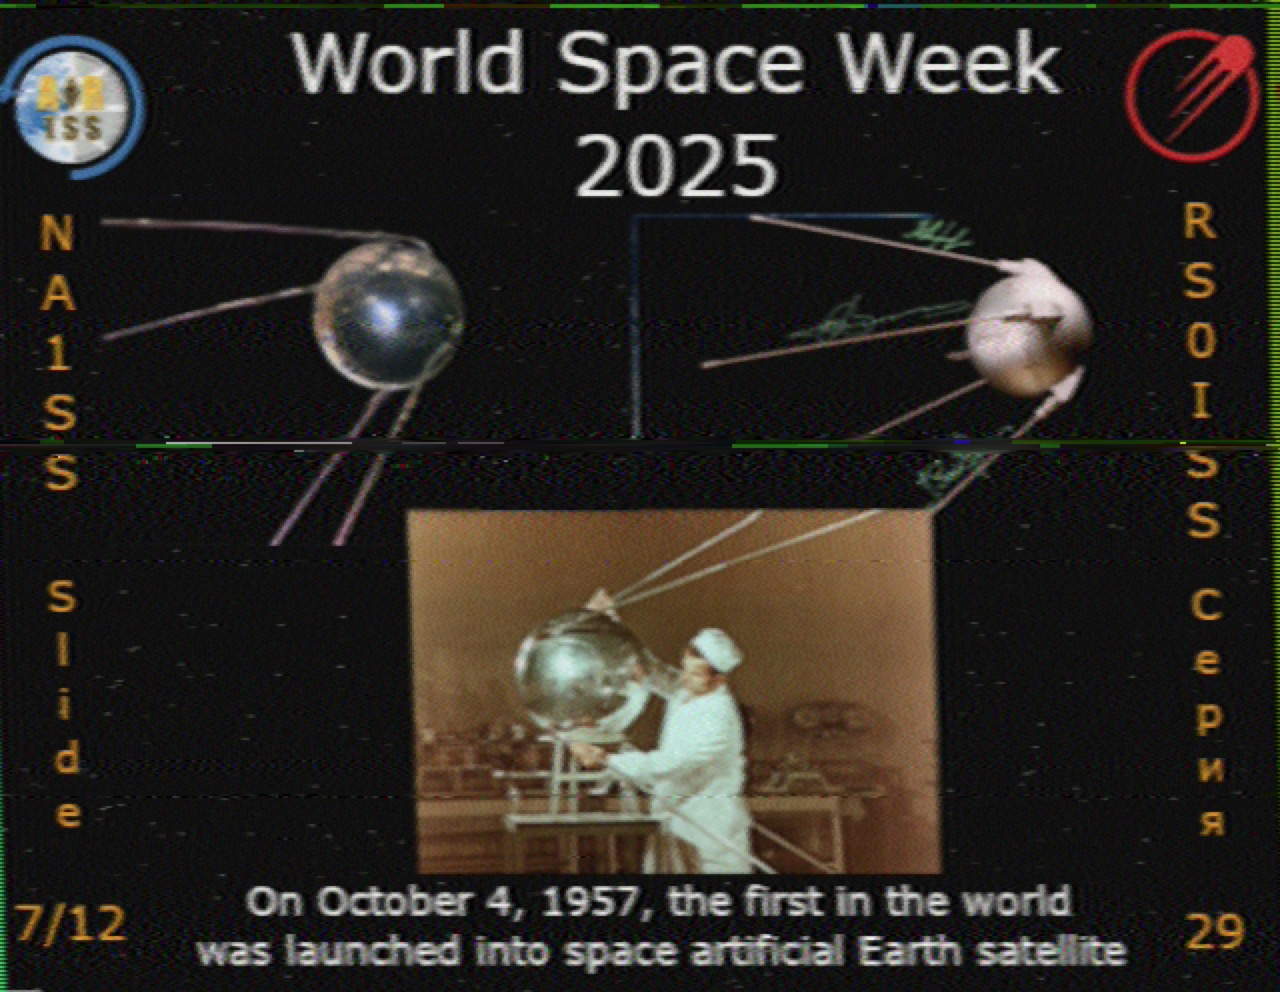
\includegraphics[scale=.15]{bilder/sstv.jpg}    
  \end{center}
  
\end{sol}


\begin{ohmchapter}
  Digitale Signale werden oft nicht direkt (nativ) vom Funkgerät verarbeitet.
  Vielmehr wird das Funkgerät im Modus SSB betrieben, die Audio Signale kommen aber natürlich nicht via Mikroton sondern werden per USB Audio interface von einem Computer erzeugt.
\end{ohmchapter}


\subsection{9600-Port }

\begin{sol}{EF219}
Wie wir im Eingang zu diesem Kapitel gelernt haben umgeht der 9600-Port den Audio Bereich des Funkgeräts und steuert direkt den Demodulator an. Der Demodulator ist zwischen 3 und 4. Wir wählen 4, da dies nach der NF Verarbeitung aber vor dem Demodulator ist.
\end{sol}

\begin{sol}{EF309}
Wir gehen analog zu Frage \qref{EF219} vor. Es kommt nur 2 in Frage, da dies nach dem NF Bandpassfilter aber vor dem Modular ist. Achtung: die Position 1 ist im NF Teil des Senders. Bitte nicht verwirren lassen.
\end{sol}

\begin{ohmchapter}
Der 9600-Port dient der schnellen digitalen Datenkommunikation (z.,B. Packet Radio, APRS) mit 9600 Baud. Er umgeht die sprachoptimierte Audioverarbeitung des Transceivers durch direkte Einspeisung analoger Audiosignale vom externen Modem/TNC in den Frequenzmodulator. Dies ermöglicht höhere Übertragungsraten im Vergleich zu herkömmlichen 1200-Baud-Verbindungen über den Mikrofonanschluss. Die übertragenen Signale sind analog (AFSK/FSK Töne), nicht digital im Sinne von TTL-Pegeln.
Damit hat der 9600-Port eine größere Bandbreite als die Anbindung via SSB die wir im vorherigen Kapitel kennengelernt haben und steuert den Modulator/Demodulator direkt an.
\end{ohmchapter}






\subsection{Übersteuerung }

\begin{sol}{EJ217}
  Wenn die ALC eingreif ist das Audio Signal zu hoch eingestellt. Dadurch kann es zu Störungen auf den Nachbarfrequenzen kommen.
\end{sol}

\begin{sol}{EJ218}
Wie schon seit Frage \qref{EJ217} bekannt wollen wir nicht, dass die ALC aktiv wird. Allerdings sollte der Pegel natürlich möglichst hoch sein. Deshalb stellen wir den Pegel genau so hoch, dass die ALC gerade so keinen Ausschlag hat. Dies können wir z.B. für den FT-8 Betrieb machen in dem wir der Audio Regler (am Computer) des Audio Interface hochdrehen und dabei die ALC beobachten. Wenn die ALC ausschlägt gehen wir mit der Lautstärke noch etwas herunter. 
\end{sol}


\begin{sol}{EJ219}
Wie in Frage \qref{EJ218} erklärt reduzieren wir den NF-Pegel (Lautstärke) noch etwas.
\end{sol}

\begin{ohmchapter}
Wir haben gelernt, dass viele Digitale Signale über ein Audio Interface und dem Transceiver im SSB Modus erzeugt werden. Wir wissen auch, dass es in SSB auf den Audio Pegel ankommt um einen störungsfreien Betrieb durchzuführen.
\end{ohmchapter}


\subsection{Automatische Empfangsberichte}
Viele Stationen Empfangen Radio Signale und verbreiten diese via Internet (WebSDR),
Besonders im digitalen Bereich könne diese Signale automatisch dekodiert werden und der Empfang kann an zentrale Server berichtet werden. Dort können sie zentral eingesehen werden.
Z.B. werden automatisiert dekodierte CW Signale vom \href{https://www.reversebeacon.net/}{Reverse Beaken Network} gesammelt.
FT8 und PSK vom \href{https://pskreporter.info}{PSK reporter}.

\begin{ohmchapter}
\end{ohmchapter}



\subsection{Paketvermittelte Netzwerke}


\begin{sol}{EE412}
Wie allgemein bekannt werden Informationen im Internet via Paketen verteilt.
Das Internet besteht dabei aus vielen kleinen Netzwerken die diese Pakete austauschen. Du hast vermutlich bei Dir zuhause einen Internet Router (in vielen Fällen ist dies eine FritzBox). Er stellt für Dich die Verbindung von Deinem lokalen Netzwerk (WLAN) zu allen anderen Netzwerken her. D.h. wenn Du an Deinem Computer eine Internetseite öffnest, werden eine oder mehrere Pakete erzeugt die zunächst alle an Deinen Router gehen. Der Leitet sie dann an das Netzwerk Deines Internet Providers weiter und solange \textbf{weitergeleitet} bis das Paket den Zielserver erreicht.
\end{sol}

\begin{sol}{EE413}
Die IP-Adresse und die Subnetzmaske definieren zusammen das lokale Netzwerk, indem sie bestimmen, welcher Teil der IP-Adresse die Netzwerk-ID (das lokale Netz) und welcher Teil die Host-ID (ein spezifisches Gerät innerhalb dieses Netzes) identifiziert.
\end{sol}

\begin{sol}{EE414}
  Für diese Frage ist die Musterantwort schlecht formuliert. Das Internet ist zunächst ein Netzwerk, dass das Internet Protokoll (IP) befolgt. Diese IP Pakete können auch mit Amateurfunk weitergeleitet werden, wobei z.B. das Rufzeichen in höheren Netzwerkebene (z.B. TCP) ausgetauscht werden. Wir merken uns die Formulierung der Musterantwort.
\end{sol}


\begin{ohmchapter}
In diesem Kapitel haben wir einige Fragen zu den Grundlagen eines \textbf{Paketvermittelten Netzwerk}. Es geht konkret um das IP-Protokoll, dass dem Internet wie Du es kennst zu Grunde liegt. Die Details verrate ich jeweils bei den Fragen.

\end{ohmchapter}


\subsection{Amplituden- und Frequenzumtastung (ASK, FSK)}

\begin{sol}{EE406}
Nur in der Musterlösung A ändert sich die Amplitude.
\end{sol}


\begin{sol}{EE407}
Nur in der Musterlösung A ändert sich die Frequenz.
\end{sol}

\begin{ohmchapter}
  Im Kapitel \ref{sec:modulation} zur Modulation hast Du bereits FM und AM kennengelernt. 
  Diese Arten der Modulation lassen sich auch auf digitale Übertragungsverfahren anwenden.
  Da die Grundlage der Modulation hier digital ist sprechen wir von einer \textbf{Umtastung}.

  \begin{description}
    \item[ASK] (Amplitude Shift Keying) oder auf Deutsch Amplitudenumtastung.
    Hier werden für 0 bzw. 1 jeweils unterschiedliche Amplituden gesendet.
    \item[FSK] (Frequency Shift Keying) oder auf Deutsch Frequenzumtastung. Es werden unterschiedliche Frequenzen gesendet. 
  \end{description}

\end{ohmchapter}

\subsection{AFSK}
\begin{ohmchapter}
Wir haben bereits ASK und FSK im letzten Kapitel kennengelernt.
Bei AFSK (Audio Shift Keying) wird das NF Signal digital umgetastet, in dem verschiedene Tonhöhen für 0 und 1 erzeugt werden. Dies wird dann z.B. via FM moduliert und gesendet (also FSK).
Ein bekanntest AFSK Signal ist z.B. APRS (Automatic Packet Reporting System), dass in Europa auf \SI{144,800}{\mega\hertz} gesendet wird.

\end{ohmchapter}

\subsection{Datenübertragungsrate}

\begin{sol}{EE401}
Wie wissen die Bandbreite wird in Hertz angegeben es geht um den genutzten Frequenzbereich. Die Datenübertragungsrate aber in Bits pro Sekunde also der Datenmenge die pro Sekunde übertragen wird.

\end{sol}

\begin{ohmchapter}
  In diesem Kapitel geht es um die Datenübertragungsrate. Wir haben im Kapitel \ref{sec:binär} zum binären Zahlensystem bereits gelernt, was ein \textbf{Bit} ist. 
  Die Datenübertragungsrate gibt einfach an wie viele \textbf{Bits pro Sekunde} übertragen werden.
\end{ohmchapter}  


\subsection{Vielfachzugriff}

\begin{sol}{EE409}
Das T in TDMA steht für \qq{time} also \textbf{Zeit}.
\end{sol}

\begin{sol}{EE410}
Das F in FDMA steht für \qq{frequency} also \textbf{Frequenz}.
\end{sol}

\begin{sol}{EE411}
Das C in CDMA steht für \qq{code}, hier geht es um  \textbf{Spreizcodes}.
\end{sol}

\begin{ohmchapter}
In der drahtlosen Kommunikation sind \textbf{Frequenzmultiplex (FDMA)}, \textbf{Zeitmultiplex (TDMA)} und \textbf{Codemultiplex (CDMA)} die zentralen Verfahren, um das gemeinsame Frequenzspektrum effizient unter mehreren Nutzern aufzuteilen und Interferenzen zu minimieren. Die Wahl des Verfahrens hängt von den spezifischen Anforderungen an Bandbreite, Nutzerzahl und Robustheit ab.

\begin{description} 
    \item[\textbf{FDMA (Frequency Division Multiple Access)}]
     \ \\
    \begin{itemize}
        \item  \textit{Funktionsweise}: Das Frequenzband wird in mehrere getrennte Frequenzkanäle unterteilt, wobei jeder Kanal einem einzelnen Nutzer fest zugewiesen wird (\textbf{Trennung über Frequenz}).
        \item \textit{Kurzcharakteristik}: Einfaches, etabliertes Verfahren; jedoch bandbreitenineffizient bei vielen Nutzern.
        \item \textit{Anwendungsbeispiele}: Analoge Mobilfunknetze (z.B. AMPS), Satellitenkommunikation.
    \end{itemize}

    \item[\textbf{TDMA (Time Division Multiple Access)}]
    \ \\
    \begin{itemize}
        \item \textit{Funktionsweise}: Alle Nutzer teilen sich denselben Frequenzkanal, erhalten aber nacheinander in festgelegten Zeitintervallen Zugriff auf den Kanal (\textbf{Trennung über Zeit}).
        \item \textit{Kurzcharakteristik}: Hohe Frequenzeffizienz; erfordert jedoch präzise Synchronisation der Zeitschlitze.
        \item \textit{Anwendungsbeispiele}: GSM (2G Mobilfunknetze), DECT.
    \end{itemize}

    \item[\textbf{CDMA (Code Division Multiple Access)}]
    \ \\
    \begin{itemize}
        \item \textit{Funktionsweise}: Alle Nutzer nutzen denselben Frequenzkanal zur gleichen Zeit. Die Trennung erfolgt über individuelle, orthogonale \textbf{Spreizcodes}.
        \item \textit{Kurzcharakteristik}: Höchste Flexibilität und Kapazität; sehr robust gegen Störungen; erfordert aber komplexe Signalverarbeitung.
        \item \textit{Anwendungsbeispiele}: UMTS (3G Mobilfunknetze), GPS.
    \end{itemize}
\end{description}

\vspace{1em}

\noindent \textbf{Zusammenfassung:} FDMA ist die einfachste Methode, während TDMA und insbesondere CDMA zunehmend effizienter und komplexer werden. CDMA bietet die größte Flexibilität bei begrenzter Bandbreite und vielen Nutzern, erfordert jedoch auch die technologisch aufwendigste Umsetzung.



\end{ohmchapter}  

\end{document}
